%
% Chapter 5
% Discussion
%

\chapter{Discussion}
\label{ch:discussion}

% TODO: check each section provides some solutions

% not so ambitious as systems immunology
% \1 <By chapter context-content-conclusion overview.>
%     \2 <ch 2: systems vaccinology study of Pandemrix>
%         \3 context: existing Sobolev study of expression differences between pandemic flu vaccine R/NR had small sample size and binary phenotype
%         \3 content: meta-analysis of existing array with new RNAseq data and continuous phenotype
%         \3 conclusion: distinct innate and adaptive expression response at d1 and d7; heterogeneity between array and RNAseq. significant expression differences between R/NR in meta-analysis at the gene set level
%     \2 <ch 3: in vivo reQTL study of Pandemrix>
%         \3 context: relatively few studies have assessed the impact of genetic variation on expression response to flu vaccine
%         \3 content: reQTL analysis for flu vaccine at d0, d1, d7. many reQTLs including sign flips. no particular gene set enrichments. evidence of cell type interactions at top hits.
%         \3 conclusion: difficult to separate out modifying effect of cell composition. this may be a fundamental flaw in the study design
%     \2 <ch 4: systems immunology and reQTL study of response to anti-TNF treatment in CD>
%         \3 context: studies on expression signatures of anti-TNF PNR have been small
%         \3 content: R/NR comparison with larger n, at baseline, w14, and over time. reQTL analysis over 4 timepoints.
%         \3 conclusion: a few hits for PNR at baseline. much stronger expression differences stronger at w14, then maintained until w54. Weak evidence for reQTLs, probably due to smaller magnitude of cell proportion changes over time vs the previous chapter.
%     \2 <discussion: limitations, future outlook>
%         \3 main themes and parallels tying together the thesis
%         \3 shared set of limitations permeating all chapters
%         \3 recommendations for future analyses and study design

Human immune response to perturbation is variable at numerous molecular and phenotypic levels.
In this thesis, I profiled the transcriptomic response to \textit{in vivo} vaccine and drug perturbations,
established associations between expression and phenotypic response,
and mapped changes in the genetic regulation of expression response over time.

\cref{ch:hird_DGE} focused on the transcriptomic response to Pandemrix vaccination in the \gls{HIRD} cohort,
describing the transition from innate to adaptive immune response,
and detecting associations between expression and antibody response.
In \cref{ch:hird_reQTL}, 
I considered the impact of host genetics on vaccine response in \gls{HIRD},
identifying genetic variants associated with changes in expression post-vaccination,
then attempting to define mechanisms that explained such associations.
Finally, \cref{ch:multiPANTS} applied similar analysis frameworks in a different context---response to anti-\gls{TNF} therapy in \gls{CD} patients in the \gls{PANTS} cohort,
finding distinct trajectories of expression between primary responders and non-responders to treatment. 

Each chapter presented its results and limitations in turn,
but similarities in design and analysis qualify them for a joint deliberation.
In this final chapter,
I highlight shared themes,
examine core limitations,
and outline considerations for the design and analysis of future longitudinal \textit{in vivo} perturbation studies
to better our biological understanding of immune response to vaccines and drugs.

\section{Design and analysis strategies for detecting robust associations}

In \cref{ch:hird_DGE,ch:multiPANTS}, I focused on identifying genes with differential expression after immune perturbation, 
or expression associated with phenotypic response variables---antibody titres and clinical anti-\gls{TNF} response respectively.
Vaccine and drug perturbation had strong effects on large proportions of the blood immune transcriptome, 
resulting in thousands of highly significant associations when comparing pre- and post- perturbation timepoints.
In comparison, it was much more challenging to identify robust single gene associations with response phenotypes.
In \cref{ch:hird_DGE}, associations of day 7 expression with antibody response from \textcite{sobolev2016AdjuvantedInfluenzaH1N1Vaccination} were replicated in my analysis of the array data, but not in \gls{RNAseq} data, or in a meta-analysis.
In \cref{ch:multiPANTS}, baseline associations with anti-\gls{TNF} from the literature---including at \gene{TREM1}, previously reported by two independent groups \autocite{gaujoux2019CellcentredMetaanalysisReveals,verstockt2019LowTREM1Expression}---were not replicated in my analysis of the \gls{PANTS} cohort.
The biological effect size of expression on response is likely to be small, eclipsed by other sources of variation: 
measurement platform, response definitions, sample characteristics, and noise.

The idealistic suggestion is to increase sample size, 
but resource and ethical constraints mean samples are often just the largest that can be feasibly obtained.
Rather than creating new cohorts, a logistically-efficient strategy is sampling from from individuals enrolled in drug and vaccine trials,
but care must be taken to ensure the trial is powered both for its primary endpoints,
and for planned transcriptomic analyses.
Power calculations for \gls{DGE} are non-trivial,
and it is often not known what a reasonable effect size to assume might be for exploratory studies.
Many experiments choose parameters like sample size and sequencing depth based on rules of thumb \autocite{conesa2016SurveyBestPractices}, or to be comparable to existing ones in the field.
% NOTE:
% https://stats.stackexchange.com/questions/176384/do-underpowered-studies-have-increased-likelihood-of-false-positives
% The basic problem with underpowered studies is that, although the rate of false positives (type I error) in hypothesis tests is fixed, the rate of true positives (power) goes down. Hence, a positive (= significant) result is less likely to be a true positive in an underpowered study. This idea is expressed in the false discovery rate [2], see also [3]. This seems what the quote refers to.
% An additional issue often named regarding underpowered studies is that they lead to overestimated effect sizes. The reasons is that a) with lower power, your estimates of the true effects will become more variable (stochastic) around their true value, and b) only the strongest of those effects will pass the significance filter when the power is low. One should add though that this is a reporting problem that could easily be fixed by discussing and reporting all and not only significant effects.
In cases where high power is not guaranteed and small effects are possible,
when reporting and interpreting associations that have been determined to be significant based on some threshold, 
one should always be cognizant of winner's curse \autocite{huang2018PowerFalseDiscovery}.
% This is doubly the case when effect sizes are known to be small,
% as years of failed replications from underpowered candidate gene studies of complex traits have demonstrated \autocite{border2019NoSupportHistorical}.
% Likely plays a part in why early systems vaccinology studies didn't include host genetics.

Another consideration is how best to distribute a fixed sample size between depth (number of individuals) and richness (number of timepoints, phenotypes, data types).
For a phenotype as dynamic as immune response, longitudinal sampling is required.
In \cref{ch:hird_DGE}, sampling demonstrated a distinct jump from day 1 innate to day 7 adaptive immune expression profiles,
but the kinetics of the transition are not clear. 
In hindsight, responses could have peaked earlier or later in different individuals,
and variation in the speed of response can not be examined without denser sampling.
In \cref{ch:multiPANTS}, expression differences between responders and non-responders were apparent from week 14, but it is not known if differences actually appear much earlier.
Future analysis of a (small) number of available samples from day 3 after initiating anti-\gls{TNF} treatment may uncover associations in the early innate response.

Rich sampling also offers analytical advantages.
Having repeated measures from the same individuals allowed modelling of within-individual covariance in \cref{ch:hird_DGE,ch:multiPANTS}, improving statistical efficiency.
The spline model in \cref{ch:multiPANTS} enabled separation of responders and non-responders based on expression trajectory over multiple timepoints.
However, in each case models only incorporated two data types: expression and phenotypic response.
Studies in the systems vaccinology field have demonstrated how integrating networks of multiple data types identifies correlates and predictors of response not only in the transcriptome, 
but in multiple layers of the immune system \autocite{li2017MetabolicPhenotypesResponse}.
In \gls{HIRD}, longitudinal \gls{FACS} and cytokine measurements are available for this form of integrative modelling.

% \1 Even if the raw number of samples goes up, subgrouping quickly attenuates the effective sample size.
%     \2 e.g. looking for timepoint, responder, cell type interactions
%     \2 pre-specify interactions of interest at the power analysis stage in design of new experiments
%     \2 for existing datasets, a workaround like the two stage strategy in ch3, assuming that interactions are only interesting at significant main effects

When transcription is quantified on a global scale, analyses should not consider genes in isolation.
% the unit of analysis should not be restricted to single genes.
Genes in the immune system are not independent, and just as variation increases uncertainty, covariation reduces it\footnote{Wickham, H. \& Grolemund, G. Chapter 7: Exploratory Data Analysis. R for Data Science. \url{https://r4ds.had.co.nz/exploratory-data-analysis.html}}.
In \cref{ch:hird_DGE}, imprecise estimates from multiple genes were used to build an informative empirical prior for between-platform heterogeneity.
Throughout the thesis, I make extensive use of enrichment analyses with gene sets defined by prior biological knowledge,
to detect subtle but coordinated changes based on the expression of multiple genes.
General purpose gene sets may be less relevant in immune cells \autocite{nakaya2015SystemsAnalysisImmunity}, 
so I used \glspl{BTM} \autocite{chaussabel2008ModularAnalysisFramework,li2013MolecularSignaturesAntibody} tailored for immune gene expression in blood.
Alternative databases that provide immune system focused gene sets include InnateDB \autocite{breuer2013InnateDBSystemsBiology} and MSigDB \autocite{liberzon2011MolecularSignaturesDatabase}.
Many significant module associations with vaccine antibody response and clinical drug response were identified in \cref{ch:hird_DGE,ch:multiPANTS},
and my expectation is that these should be more replicable than any single gene associations I reported (e.g. \gene{SIGLEC10} from \cref{ch:multiPANTS}).
While the effect size of a single gene may vary from sample to sample due to noise, 
a summary measure computed from multiple genes should be more robust.
Indeed, some module associations between baseline expression and antibody response found in \cref{ch:hird_DGE} were reported in previous studies of seasonal influenza vaccines.
Most systems vaccinology studies aiming to identify consistent associations with vaccine response over multiple cohorts and sampling years focus their analyses at the gene set level \autocite{tsang2020ImprovingVaccineinducedImmunity}.
Gene set analyses cannot, however, be divorced from examining the genes within them,
as the genes that drive set associations can differ between apparent replications,
and the mapping between genes and sets is one-to-many.

\section{Responder analysis}
\label{sec:discussion_responderAnalysis}

A key determinant of how well the models in this thesis might correspond to reality lies in the assumed model for phenotypic response.
By encoding response as an independent variable, an assumption is made that it is a stable characteristic of an individual that is measured without error%
\footnote{The regression framework can accommodate measurement error in the context of errors-in-variables models.}.
This may not be an accurate assumption.
Imagine a hypothetical drug or vaccine where 60\% of a sample of individuals have an observed response phenotype: \enquote{60\% of the time, it works every time}\footnote{Apatow, J., McKay, A. \& Ferrell, W. Anchorman: The Legend of Ron Burgundy (2004).}.
This is compatible with a stable 60\% success rate in 100\% of individuals (variation in observed response is entirely due to chance);
or a stable 100\% success rate in 60\% of individuals and 0\% in the other 40\% (response is highly personal)---most likely the truth is somewhere in between.
In the first scenario, it is difficult to imagine identifying robust baseline associations with response.
This has been extensively discussed in the context of randomised controlled trials \autocite{senn2018StatisticalPitfallsPersonalized}, 
but similar issues pertain to response definitions in observational studies.

One needs to establish how correlated phenotypic response is over time within the same individual,
\todo{I mean phenotypic response here, not (biological or technical) variation in expression measurements}
and to compute within-individual variation requires replication at the level of the individual.
% \2 also applies to continuous measures of response, as what is being considered is that it only makes sense to talk about response if the response measure is tightly correlated within an individual over time
The same individual must be \emph{perturbed and measured} more than once \autocite{senn2016MasteringVariationVariance}.
This is not always possible in practice.
In \cref{ch:hird_DGE}, antibody response was defined based on a single measurement after a single dose.
but measuring response after a hypothetical second dose would quantify a different phenotype: 
the secondary immune response based on vaccine-induced immune memory.
In \cref{ch:multiPANTS}, all patients received repeated doses interspersed with sampling timepoints,
and the expression differences between clinical responders and non-responders seen at week 14---the timepoint where clinical response was assessed---were maintained at week 30 and week 54,
suggesting the initial designation of non-responders is not due to chance, but due to some characteristic of patient disease state.
%
% \2 note for the specific case of genetic factors, the field of complex trait genetics has long had a solution for this: twin studies are analogous to measuring the same individual twice
%     \3 For phenotypes like vaccine response in ch2 that can be, twin studies have already demonstrated heritability of certain response phenos like influenza vaccine Ab titres \autocite{brodin2015VariationHumanImmune}
%     \3 In pharmocogenetics, twin studies are less common \url{https://www.sciencedirect.com/science/article/abs/pii/S0928098719300326} and have not been done for response to anti-TNFs (the ch4 setting)
%     \3 repeated crossover trials can be a feasible alternative to twin studies \url{https://www.researchgate.net/profile/Laszlo_Endrenyi/publication/13553486_Hypothesis_Comparisons_of_inter-_and_intra-individual_variations_can_substitute_for_twin_studies_in_drug_research/links/59e97c2e458515c36370e6a7/Hypothesis-Comparisons-of-inter-and-intra-individual-variations-can-substitute-for-twin-studies-in-drug-research.pdf} \autocite{senn2016MasteringVariationVariance}

Even if response is actually a stable personal characteristic, one still needs to select an appropriate mathematical definition.
As discussed in \cref{subsec:hird_dge_TRI}, a binary definition of response based on dichotomisation is inefficient and biologically implausible.
I instead used the \gls{TRI} in \cref{ch:hird_DGE,ch:hird_reQTL}, a continuous change score combining \gls{HAI} and \gls{MN} titres, residualised on the baseline titres.
In \cref{ch:multiPANTS}, the binary clinical response phenotype is based on a complex decision tree with many inputs.
Defining dichotomies based on multiple inputs can lead to discontinuities and non-monotonicity in response probabilities under small changes in inputs \autocite{senn2005DichotomaniaObsessiveCompulsive}.
Pragmatism did come into play when choosing these definitions.
For \gls{DGE}, the simplest models encode phenotypic response variable as a single independent variable, with expression as the sole dependent variable.
Both \gls{TRI} and the \gls{PANTS} clinical response definition provided that single independent variable.
In hindsight, variation in response definitions likely contributes to difficulties in replicating associations between studies,
so it may be more sensible to model on the components phenotypes themselves (e.g. log \gls{HAI} and \gls{MN} titres, \gls{CRP} levels and \gls{HBI} scores).

% \1 bias in non-randomised studies
    % \2 In RCTs, the treatment effect would be defined against the effect in the control group
    % \2 In prospective cohort studies, the treatment effect is determined between two subgroups within the cohort

\section{Challenges in the interpretation of bulk expression data}

Bulk expression data is a mixture of cell types with heterogeneous expression profiles.
One of the largest sources of variation in bulk blood expression data is variation in immune cell composition, generated from true variation in composition and sampling effects.
The more cell type-specific a gene's expression, the more its measurement in bulk is affected by cell composition \autocite{farahbod2020UntanglingEffectsCellular}.
Highly cell type-specific genes can be treated as marker genes, 
used in deconvolution methods to estimate cell proportions in bulk samples when they are not directly measured.
In \cref{ch:hird_reQTL}, xCell---while not technically a deconvolution method---was used to estimate cell type enrichment scores from array and \gls{RNAseq} data.
In \cref{ch:multiPANTS}, estimates of cell proportions were computed by deconvolution of matched genome-wide methylation data.
When fit as covariates in linear regression, 
cell abundance estimates act as precision variables for sampling noise, 
but additionally as mediators of the perturbation's effect on expression.
% Many \gls{DGE} and \gls{eQTL} mapping methods require the same set of covariates for all genes.
In \cref{ch:multiPANTS}, I chose to run two sets of models with and without including estimates of five major immune cell proportions,
gaining some information on which effects are driven by cell abundance, and which are driven by per-cell up or downregulation.

Using major cell populations for correction misses the contribution of rare populations \autocite{pellegrinocoppola2020CorrectionBothCommon}.
For cis-\gls{eQTL} mapping in \cref{ch:hird_reQTL,ch:multiPANTS}, where the main concern was maximising the number of \gls{eQTL} detected,
hidden factors from PEER were included into models in addition to known cell abundance estimates.
PEER factors were correlated with known cell abundance, so it is likely they capture additional variation from rarer cell types.
If having interpretable covariates for cell abundance is unimportant,
methods like surrogate variable analysis \autocite{leek2014SvaseqRemovingBatch,liu2016EvaluationMethodsRemoving}
can be used to adjust for cell composition and other unmeasured technical sources of variation in \gls{DGE} also.

Interpretable covariates for cell abundance are important for considering \gls{reQTL} effects in bulk data.
As discussed in \cref{subsec:hird_reQTL_methods_cellTypeInteraction}, 
it is model misspecification to omit genotype-cell abundance interactions if the effect of genotype changes depending on cell abundance.
In fact, it is popular to use such interaction terms between genotype and cell abundance (or a proxy of cell abundance) 
to discover cell type-specific \gls{eQTL} \autocite{westra2015CellSpecificEQTL,kim-hellmuth2020CellTypeSpecific}.
\textit{In vivo}, cell abundances are causally affected by the perturbation, due to active recruitment, differentiation, proliferation of immune cells.
Consider the case where vaccine perturbation causes active proliferation of a rare cell type that is near absent at baseline, 
but forms a greatly increased proportion of the bulk mixture after perturbation.
Any baseline \gls{eQTL} specific to this cell type will appear as a \gls{reQTL} in the post-perturbation timepoint, 
because expression of that cell type contributes more to the bulk mixture.
If the eGene is not cell type-specific in its expression, 
adjusting for abundance of the cell type will only offset the regression lines at each timepoint, but not change their slopes relative to one another.
The eGene also does not have to be upregulated on average, 
as the effect of interest is genotype on the pre-post difference in expression, not the difference itself.
In \cref{ch:hird_reQTL}, I found that an increase in naive classical monocytes at day 1 revealing a
non-stimulus-specific but monocyte-specific \gls{eQTL},
for the non-monocyte-specific gene \gene{ADCY3},
% even though the expression of \gene{ADCY3} is not monocyte-specific,
% and \gene{ADCY3} is not upregulated,
was a plausible mechanism underlying the strongest day 1 \gls{reQTL}.

An aim of the \textit{in vivo} \gls{reQTL} design is to find host genetic variants with a causal effect on response to perturbation.
The crux of the issue is whether such an interpretation is justifiable: whether a difference in group-level \gls{eQTL} regression slopes between baseline and post-perturbation
necessarily entails a causal effect of genotype on change in expression from baseline to post-perturbation at the individual level.
For the specific case of \gene{ADCY3} day 1 \gls{reQTL}, I believe so.
Individuals homozygous for the effect allele do tend to have strongly increased expression at day 1.
Individuals homozygous for the non-effect allele do tend to have decreased expression at day 1.
If you were to change the genotype of an individual from homozygous effect to homozygous non-effect,
you \textit{would} change their post-vaccination increase of \gene{ADCY3},
because the exact same increase in monocyte count from baseline to day 1
would provide fewer \gene{ADCY3} transcripts.
The effects cancel on average, thus the gene is not differentially expressed between day 1 and baseline overall.
% There may indeed be some causal effect of genotype on ability to
% TODO: actually measure is not expression, but some proportion...

In the general case, I am unsure.
There are many possible mechanisms at each \gls{reQTL}:
a gene with an \gls{eQTL} not expressed at baseline becoming detectable (power),
a cell type with a cell type-specific \gls{eQTL} increasing in proportion (recruitment or proliferation),
a effect of a cell type-specific \gls{eQTL} increasing within that cell type (activation, the canonical scenario for \textit{in vitro} stimulation),
a genotype-dependent increase in cell abundance creating a \gls{reQTL} for a gene with cell type-specific expression,
\textit{et cetera}.
Not all of these can be ruled out just by including cell abundances as covariates in the \gls{eQTL} model.
Even if a large number of \gls{reQTL} can be detected by statistical interaction, as in \cref{ch:hird_reQTL},
the challenge is distinguishing these mechanistic scenarios to form causal hypotheses.
% \2 one could imagine crude ways to falsify each hypothetical model e.g. interaction/coloc with each cell type (ch3), but always at risk of missing a cell type
It is also unclear whether \textit{in vivo} \gls{reQTL} provide additional utility over \textit{in vitro} \gls{reQTL} for gene prioritisation at \gls{GWAS} loci.
Theoretically, there may be effects unobservable without \textit{in vivo} interactions in the immune system, 
but a systematic comparison of \gls{reQTL} detected in \textit{in vivo} and \textit{in vitro} stimulation experiments has not been performed.
\textit{In vivo} \gls{reQTL} studies are certainly not ineffectual at their stated goals, 
but cell composition does add considerable complexity to their interpretation.
Although insights into the biological mechanism of the stimulation response is easier to gain when cell type abundance is controlled \textit{in vitro},
a basic utility of \textit{in vivo} stimulation is allowing the detection of additional cell type-specific \gls{eQTL} effects in bulk data using genotype-cell type abundance interaction terms;
a methodology already well-established in non-stimulated bulk samples (e.g. \autocite{westra2015CellSpecificEQTL}).

% \2 control is not intervention
% http://bayes.cs.ucla.edu/PRIMER/ch3-preview.pdf
% The difference between intervening on a variable and conditioning on that variable should,hopefully, be obvious.
% When we intervene on a variable in a model, we fix its value.
% We change the system, and the values of other variables often change as a result.
% When we condition on a variable, we change nothing; we merely narrow our focus to the subset of cases in which the variable takes the value we are interested in.
% What changes, then, is our perception about the world, not the world itself.
To truly control for cell composition, the best option is to control it at the study design stage.
Adjusting for cell abundance in regression only attempts to estimate the effect of other predictors if cell abundance were held constant.
It does not change the cell abundances to be equal---it is a change of viewpoint, not a change of data.
Adjusting for abundance also cannot distinguish cell types with correlated abundance estimates.
\Gls{scRNAseq} after \textit{in vivo} perturbation would quantify per-cell expression and cell abundance simultaneously.
The technology is emerging as an alternative to bulk sequencing of \gls{FACS}-sorted cells, with comparable cost,
and the additional advantage of not requiring pre-defined marker sets \autocite{vanderwijst2020SinglecellEQTLGenConsortium}.
There is flexibility in choosing to conduct \gls{DGE} and \gls{eQTL} mapping within each cell type cluster, or to pool clusters to mimic bulk data.
Paired designs that leverage the power of bulk \gls{reQTL} mapping and the cell type resolution of single-cell data have been explored,
using eGene expression in clusters to annotate bulk \gls{reQTL} to likely cell types \autocite{devries2020IntegratingGWASBulk}.
As an emerging technology, \gls{scRNAseq} still faces many limitations, such as
    low coverage of the transcriptome due to drop out, 
    smaller sample sizes due to cost,
    difficulties in defining robust cell type clusters,
    and sample processing effects on the transcriptome,
but progress in the field has been nothing but rapid.

% more n allows more phenotypes
%
%         disease specific biobanks e.g. ibd bioresource/predicct
%
%    Our GWASfor 54 functionally relevantphenotypes oftheadaptiveimmune system in 489 healthy individuals identifieseight genome-wide significant associations explain-ing 6%–20% of variance.
%         https://www.cell.com/cell-reports/pdf/S2211-1247(18)31493-1.pdf
%
%     PheWAS\autocite{verma2017CurrentScopeChallenges}
%         https://onlinelibrary.wiley.com/doi/full/10.1111/imm.12195
%         PheWAS has the advantage of identifying genetic variants with pleiotropic properties.
%
% and Many more conditions
    % e.g. 250 condition ASE % https://www.ncbi.nlm.nih.gov/pmc/articles/PMC5131815/
    % e.g. StructLMM
    %     Identifies eQTLs with GxE, where the number of environments in E is large (modelled as a random effect)

\section{From association to prediction}

In the \gls{DGE} regression models I used to test for association of expression with phenotypic response,
expression was always placed as the dependent variable, 
and response as an independent variable.
In a clinical setting, a more relevant concern is prediction of patient response from expression (ideally baseline expression),
reversing the roles of expression and response in the model.
In \cref{ch:hird_DGE,ch:multiPANTS},
I observed few significant single-gene associations with response at baseline.
It is first useful to consider what implications this has on the move from association from prediction in this data.

Prediction from genome-wide transcriptomic data is currently a $p \gg n$ prediction problem,
where the number of potential predictors p dwarfs the sample size n.
\textcite{efron2020PredictionEstimationAttribution} provides a fascinating case study on predicting prostate cancer status from expression array data (p=6033 genes) in 
samples from 52 prostate cancer patients and 50 controls (n=102).
After randomly splitting the data into training and test sets, each with 26 cancer patients and 25 controls,
a random forest used to predict cancer status from gene expression recorded a 2\% test set error.
Repeating over many random splits showed this high predictive performance was not an outlier.
Random forests have embedded feature selection, assigning their predictors an importance score, 
with a positive importance score indicating that a predictor was utilised by the model.
After removing all 348 genes with positive importance scores in the first model from the dataset and repeating the process with remaining p=5685 n=102 matrix,
another model was produced where a set of 364 genes with positive importance---completely disjoint from the first 348---predicted cancer status with a \emph{similar error rate}.
This process could be repeated multiple times, each time producing a model with similar error rate, using none of the \enquote{important} genes from the previous models.
The performance of pure prediction models appears to be dominated by the confluence of many weak predictors,
thus it is still feasible to consider prediction in datasets where attribution of significance to individual strong predictors may be impossible.

A large part of systems vaccinology in the last decade has been building models to predict vaccine-induced antibody and cellular responses from high-dimensional data.
The methods used span the full gamut of traditional and modern machine learning algorithms, including
classification to nearest centroid (ClaNC) \autocite{querec2009SystemsBiologyApproach},
discriminant analysis via mixed integer programming (DAMIP) \autocite{querec2009SystemsBiologyApproach,nakaya2011SystemsBiologyVaccination,nakaya2015SystemsAnalysisImmunity,kazmin2017SystemsAnalysisProtective},
nearest shrunken centroid algorithm (PAM) \autocite{vahey2010ExpressionGenesAssociated},
linear regression \autocite{bucasas2011EarlyPatternsGene,li2017MetabolicPhenotypesResponse},
logistic regression \autocite{haynes2012ImmuneCorrelatesAnalysisHIV1,furman2014SystemsAnalysisSex,tan2014GeneSignaturesRelated},
linear discriminant analysis (LDA) \autocite{zak2012MerckAd5HIV,tsang2014GlobalAnalysesHuman},
elastic net \autocite{furman2013ApoptosisOtherImmune},
partial least squares (PLS) \autocite{tsang2014GlobalAnalysesHuman},
artificial neural networks (ANN) \autocite{nakaya2015SystemsAnalysisImmunity},
naive Bayes \autocite{fourati2016PrevaccinationInflammationBcell},
lasso \autocite{qi2016DefectiveMemoryCell},
sparse partial least squares (SPLS) \autocite{rechtien2017SystemsVaccinologyIdentifies},
and logistic multiple network-constrained regression (LogMiNeR)
\autocite{avey2017MultipleNetworkconstrainedRegressions,avey2020SeasonalVariabilityShared}.
The choice of methodology can be daunting.
Fortunately (or unfortunately), 
an extensive survey of transcriptomic prediction models by the MicroArray Quality Control Consortium \autocite{maqcconsortium2010MicroArrayQualityControl}
% DA, discriminant analysis; Tree, decision tree; NB, naive Bayes; KNN, K-nearest neighbors; SVM, support vector machine.
found the choice of algorithm to be not as influential on predictive performance as 
% rigour during the model building process, and
the endpoint itself, with some endpoints being inherently difficult to predict.
% 3 points:
% simple regression-based models are a good starting point,
% domain-specific prior knowledge can be incorporated to improve performance,
% and ensemble models that combine multiple algorithms had consistently good performance and robustness.
There is also no need to restrict oneself to a particular method;
ensemble models that combine multiple algorithms consistently have the best performance and robustness \autocite{camacho2018NextGenerationMachineLearning}.
It is hard to say \textit{a priori} whether antibody response in \gls{HIRD} and anti-\gls{TNF} response in \gls{PANTS} are \enquote{difficult} endpoints.
The existence of predictive signatures for seasonal influenza vaccine response using baseline expression, 
validated over multiple cohorts, years, and geographical locations does set an encouraging precedent for the former \autocite{hipc-chisignaturesprojectteam2017MulticohortAnalysisReveals}.
% Well-implemented internal validation by repeated cross-validation or bootstrapping was comparable to estimating performance to external validation with a blinded test set,
% but nevertheless overestimated model performance.
%

Oncology was one of the earliest fields to adopt predictive gene signatures into clinical practice.
Despite the first commercial tests launching in the early 2000s (e.g. MammaPrint, a 76-gene signature for breast cancer prognosis),
only a handful are in use today \autocite{chibon2013CancerGeneExpression,michiels2016StatisticalControversiesClinical,kwa2017ClinicalUtilityGeneexpression}. 
There are multiple hurdles to clinical implementation,
requiring that a signature not only have validated accuracy, 
but provide sufficient incremental value on top of existing clinical markers in a cost-effective manner \autocite{michiels2016StatisticalControversiesClinical}.
% three main categories of feature selection algorithms: wrappers, filters and embedded methods.
% https://academic.oup.com/bioinformatics/article/23/19/2507/185254
Feature selection is of particular importance when building models for the clinic; 
cost-effectiveness entails that most expression tests are qPCR-based tests that measure at most a few dozen genes.
There is an interesting tension between the sparsity assumed by feature selection methods---that most predictors have no effect---and the observation that prediction algorithms depend on many weak predictors.
A balance between predictive performance and cost will likely need to be struck.
The ability to predict individual response to anti-\gls{TNF} treatment would be revolutionary due to the cost and quality of life impact of taking ineffectual biologic therapy.
The case for personalised vaccinology lies mostly in building understanding of the best type, dose and timing for vaccination of challenging populations \autocite{poland2018PersonalizedVaccinologyReview}.

% What sample size?
%
% https://www.bmj.com/content/368/bmj.m441
% Calculating the sample size required for developing a clinical prediction model

\section{From association to causality}

Knowing the causal mechanisms of immune response to perturbation are crucial for conceiving of possible interventions.
For example, assuming the baseline association of \gene{SIGLEC10} with anti-\gls{TNF} response identified in \cref{ch:multiPANTS} is real,
would intervening on baseline \gene{SIGLEC10} expression affect probability of response?
The study designs used in this thesis are uncontrolled, but still provide useful guarantees against reverse causality:
post-perturbation phenotypic or expression measurements cannot cause baseline gene expression,
and neither can cause genotype.
To estimate causal effects of expression on phenotype,
what is needed are models that encode causal relationships as testable hypotheses.
There are several families of such methods, and as I shall now describe, they should be used in combination.

% NOTE: nice intros
%
% https://www.biorxiv.org/content/10.1101/2020.07.01.182097v1.full.pdf
% Probabilistic Colocalization of Genetic Variants from Complex andMolecular Traits:  Promise and Limitations
%
% \autocite{zheng2020PhenomewideMendelianRandomization}
% Predicted associations between proteins and phenotypes may indicate four
% explanations: causality, reverse causality, confounding by LD between the
% leading SNPs for proteins and phenotypes or horizontal pleiotropy
% (Supplementary Fig. 3). Given these alternative explanations, we conducted a
% set of sensitivity analyses to evaluate whether each MR association reflected
% a causal effect of protein on phenotype: tests of reverse causality using
% bidirectional MR22 and MR Steiger filtering;23,24 heterogeneity analyses for
% proteins with multiple instruments25; and colocalization analyses26 to
% investigate whether the genetic associations with both protein and phenotype
% shared the same causal variant (Fig. 1).
%
% \autocite{taylor2019IntegrativeAnalysisGene}
% MR is a statistical framework that uses a genetic association (“the
% instrument”) for one trait (“the exposure”) to test for a causal
% influence on another trait (“the outcome”).  An MR result, in which the
% exposure instrument is associated with the outcome, can arise under four
% distinct models (10, 11): (i) there is no causal relationship, but a SNV
% that influences the outcome is in linkage disequilibrium (LD) with a SNV
% that influences the exposure; (ii) the exposure causally influences the
% outcome; (iii) the outcome causally influences the exposure (a reverse
% causal relationship); or (iv) the exposure and outcome are not causally
% related but share a SNV that influences both the exposure and the outcome
% independently (horizontal pleiotropy).
%
% hemani2018EvaluatingPotentialRole
% Genetic mediation-based analyses (37–40) are more liable to problems of
% confounding and measurement error than MR (41–43), but could potentially
% separate between vertical and horizontal pleiotropy in some scenarios.
% Use genetic colocalization to eliminate possibility distinct causal variants
% (25,30,31); if instruments are available for the outcome then test the reverse
% causal effect (110); if not use MR Steiger (43); use genetic mediation-based
% analysis (40,111) to try to separate horizontal and vertical pleiotropy

% NOTE: https://www.ncbi.nlm.nih.gov/pmc/articles/PMC7221461/
% has the nicest MR diagrams to copy.
\gls{MR} is a form of \gls{IV} analysis that uses genetic variants as \glspl{IV} to estimate the causal effect of an exposure on an outcome.
Three assumptions define a valid genetic \gls{IV} \autocite{daveysmith2014MendelianRandomizationGenetic,hemani2018EvaluatingPotentialRole,neumeyer2020StrengtheningCausalInference}.
In this case where the exposure is gene expression, and the outcome is some phenotypic response such as antibody titre,
the first assumption (IV1) is that variant should be associated with the exposure as an \gls{eQTL}.
% There is no need for a causal relationship; the \gls{eQTL} does not need to be fine mapped \autocite{daveysmith2014MendelianRandomizationGenetic,burgess2018InferringCausalRelationships}.
The term \gls{MR} comes from an analogy to randomised controlled trials;
meiotic segregation is largely independent of environmental confounders, 
so different \gls{eQTL} alleles can be thought to randomly assign different \enquote{doses} of expression \autocite{daveysmith2014MendelianRandomizationGenetic}.
The second assumption (IV2) is that the variant is not associated with unmeasured confounders of the expression-phenotype association, such as ancestry.
The third assumption (IV3) is that the variant has no association with phenotype except through expression. 
Combined, these assumptions place expression as complete mediator (vertical pleiotropy) of the effect of the \gls{eQTL} on phenotype (\cref{fig:discussion_MR_assumptions}).
The effects of variant on expression and expression on phenotype can be estimated in the same sample, 
or in non-overlapping samples (two-sample \gls{MR} \autocite{hemani2018EvaluatingPotentialRole,neumeyer2020StrengtheningCausalInference}).
Two-sample \gls{MR} can leverage existing large \gls{eQTL} catalogues,
and avoids weak-instrument bias, where using \gls{eQTL} with weak effects on expression biases the estimate of the expression-phenotype effect away from the null in single-sample \gls{MR} \autocite{daveysmith2020MendelLawsMendelian}.
%
% Interpretation of TWAS and its vulnerabilities
% https://sashagusev.github.io/2017-10/twas-vulnerabilities.html
A related family of methods,
\glspl{TWAS} \autocite{gusev2016IntegrativeApproachesLargescale},
train predictive models of expression from \gls{eQTL} data, 
then apply those models in \gls{GWAS} cohorts to test the association of genetically-predicted expression with phenotype.
\gls{TWAS} methods have methodological similarities to two-sample \gls{MR} \autocite{zhu2020TranscriptomewideAssociationStudies}.

% NOTE: nice figure in https://genomemedicine.biomedcentral.com/articles/10.1186/s13073-019-0613-2/figures/1
\begin{figure}
    \centering
    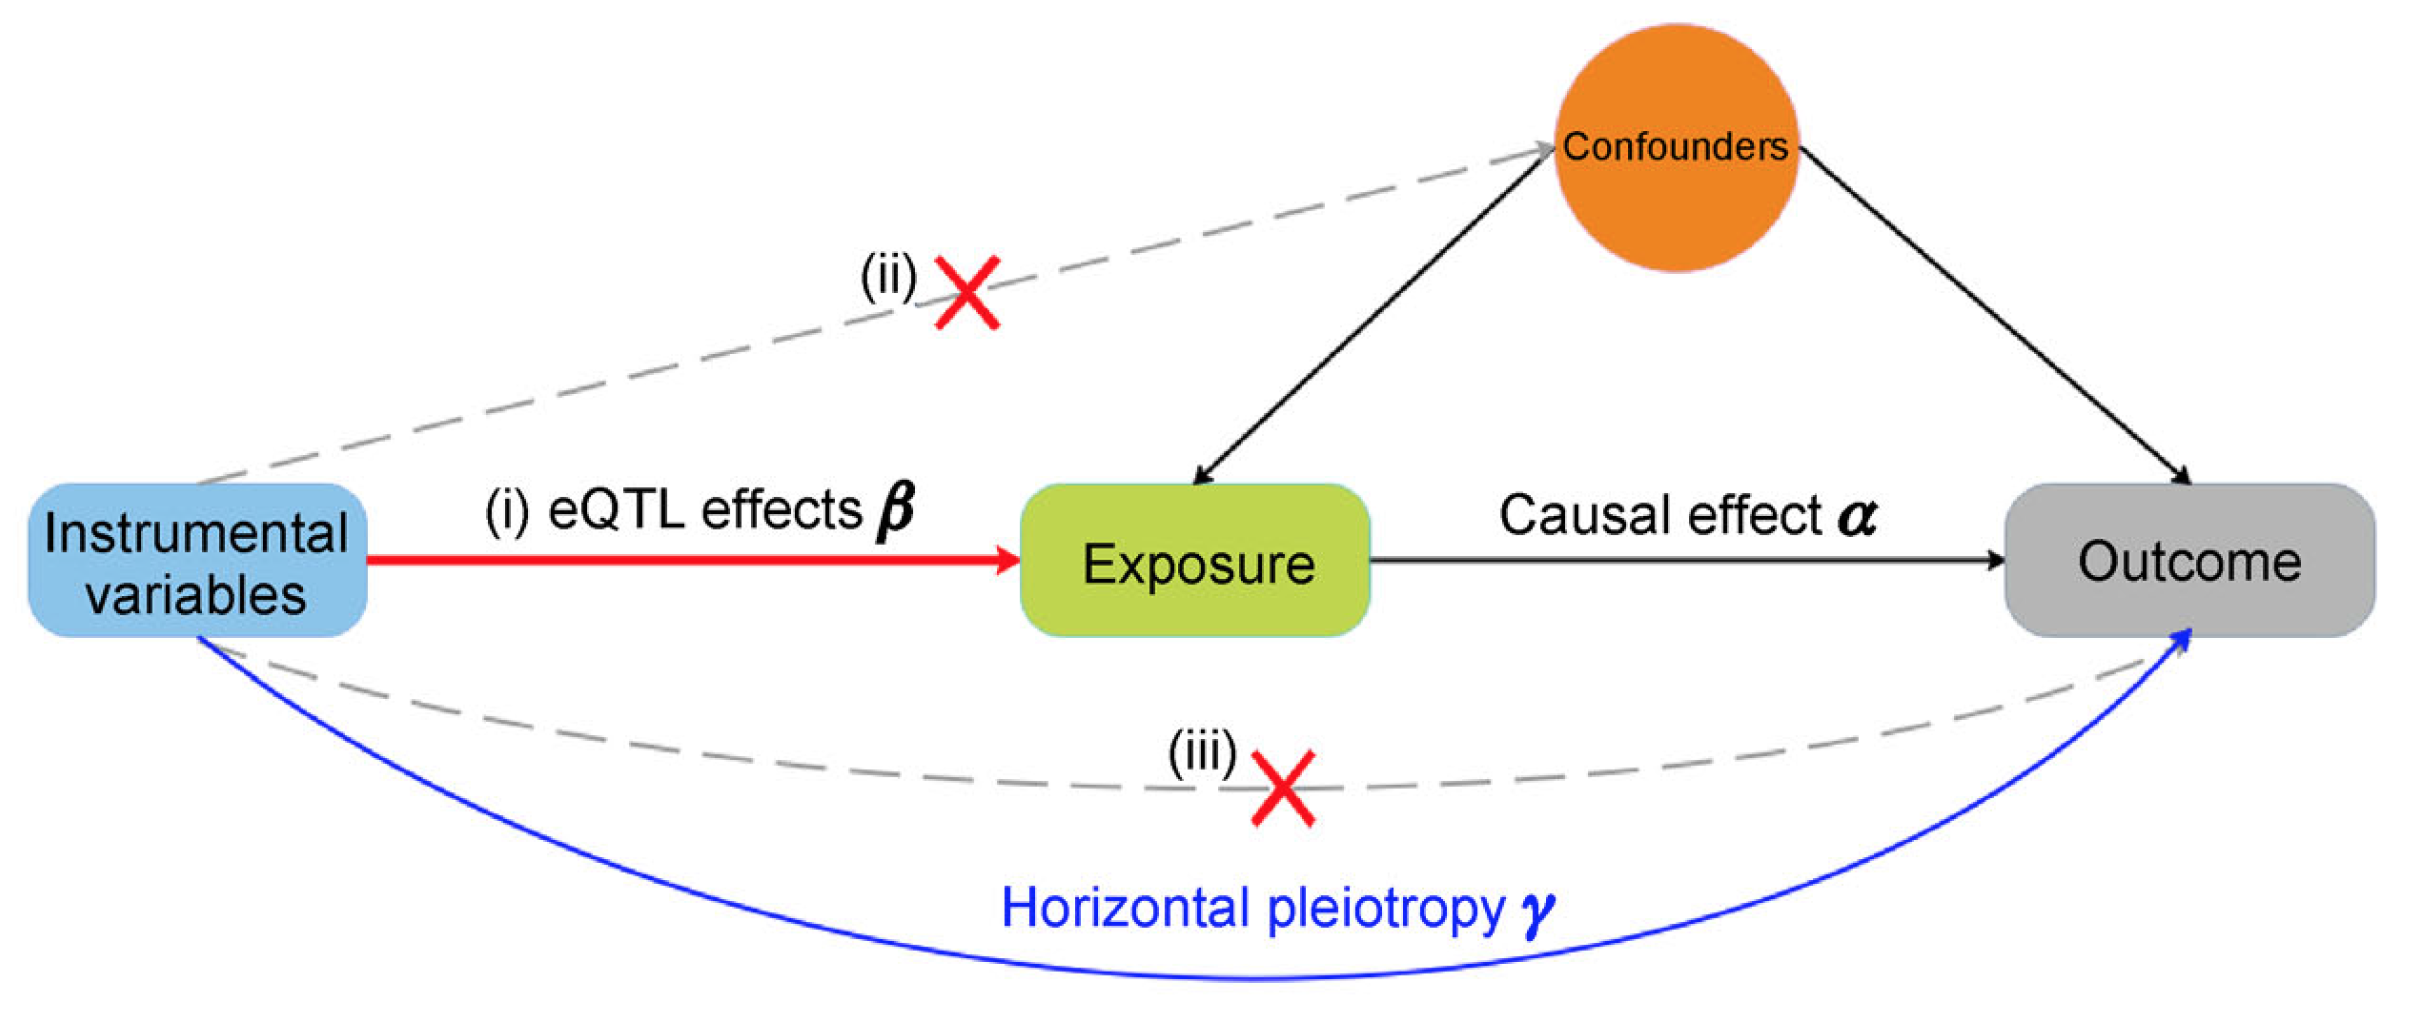
\includegraphics[width=0.9\textwidth,page=1]{mainmatter/figures/chapter_05/zhu2020TranscriptomewideAssociationStudies/Screenshot 2020-11-27 at 22.54.30.png}
    \caption{
        \textbf{The three assumptions of \gls{MR}.} 
        \gls{MR} uses genetic \glspl{IV} to estimate the causal effect \textalpha of an exposure (here, gene expression) on an outcome, under three assumptions:
        (i) IV1: the variant is associated with the exposure (here, an \gls{eQTL});
        (ii) IV2: the variant is not associated with any unmeasured confounders;
        (iii) IV3: the variant is not associated with the outcome except through exposure.
        The directionality of the arrows in the causal diagram are also assumed to hold.
        The blue arrow shows a horizontal pleiotropic effect of the variant on outcome, a violation of the IV3 assumption.
        Figure reprinted by permission from Springer Nature: Springer Nature, Quantitative Biology, \textcite{zhu2020TranscriptomewideAssociationStudies}, \textcopyright~2020.
    }
    \label{fig:discussion_MR_assumptions}
\end{figure}

Violation of \gls{MR} assumptions can result in estimating a causal effect of expression on phenotype where there is none.
The most troublesome assumption of \gls{MR} is IV3.
If there is no temporal ordering of exposure and outcome,
for instance, when evaluating the causal effect of day 7 post-vaccination gene expression on day 7 CD4\textsuperscript T cell abundance,
IV3 can be violated by reverse causation,
where the association between variant and expression might be mediated by the cell abundance phenotype.
If this is suspected, 
recommendations include performing \gls{MR} in the reverse direction if there are available instruments for the phenotype (bi-directional MR),
and extensions that test the directionality based on variance explained (MR Steiger) \autocite{daveysmith2014MendelianRandomizationGenetic,hemani2017OrientingCausalRelationship,hemani2018EvaluatingPotentialRole,neumeyer2020StrengtheningCausalInference}.
% \2 also incorporate biological knowledge, e.g. if eQTL variant is in a TF motif for a gene, more likely G -> E than G -> pheno -> E

IV3 can be violated by linkage if the eQTL does not actually have any effect on the phenotype at all, 
but simply is in \gls{LD} with another variant that does;
and can also be violated by the existence of horizontal pleiotropy, 
where the effect of the variant on expression and phenotype are independent (\cref{fig:discussion_MR_assumptions}).
Colocalisation methods, as used in \cref{ch:hird_reQTL}, can be used to test whether the same causal variant affects expression and phenotype, distinguishing pleiotropy from linkage;
however, colocalisation is necessary but not sufficient for mediation,
thus does not distinguish mediation (vertical pleiotropy) from horizontal pleiotropy \autocite{hemani2018EvaluatingPotentialRole}.
%
% Mediation can exist in the absence of a 'significant' total effect G -> pheno
% http://davidakenny.net/cm/mediate.htm
% In the opinion of most though not all analysts, Step 1 is not required. (See the Power section below why the test of c can be low power, even if paths a and b are non-trivial.)
Mediation analysis methods (e.g. CIT \autocite{millstein2009DisentanglingMolecularRelationships}, Findr \autocite{wang2017EfficientAccurateCausal}) can be used to test for violations of IV3 by horizontal pleiotropy.
They distinguish mediation from horizontal pleiotropy using comparison of causal models with different structures,
but require individual level data, and are more susceptible to measurement error than \gls{MR} \autocite{hemani2017OrientingCausalRelationship,hemani2018EvaluatingPotentialRole}.
%
% \autocite{porcu2019MendelianRandomizationIntegrating}
% Pleiotropy could alternatively be tackled using multivariable MR. If a variant exhibits horizontal pleiotropy, but we know its association(s) to some mediators of its indirect effect to the outcome, those mediators could be included as additional exposures and one can perform a multivariable MR, which can mitigate bias by jointly estimating the causal effects of all exposures on the outcome23,24.

% Canalisation/compensation and population stratification affects MR with genetic instruments also.
% https://www.nature.com/articles/s41576-018-0020-3
% https://spiral.imperial.ac.uk/bitstream/10044/1/23560/2/SIM%202015_Accepted%20version.pdf
    % The most likely cause of violation of the third IV assumption is pleiotropy,  which occurswhen a genetic variant influences multiple intermediate phenotypes that separately affectthe outcome of interest.
    % The assumption can be violated through other mechanisms includ-ing canalization and population stratification.
    % Developmental canalization occurs when agenetic variant expressed during fetal development or post-natal growth stimulates compen-satory processes that protect against the effect of that variant on the outcome in adulthood[1], while population stratification occurs when ancestral sub-populations with different al-lele frequency and outcome distributions confound theG−Yassociation [1, 5, 6].

\section{Triangulation}

Triangulation is the use of methods with different assumptions, biases, and limitations that address the same question \autocite{munafo2018RobustResearchNeeds}.
An example from this thesis appears in \cref{ch:hird_reQTL}, 
combining \gls{DGE}, between-individual \gls{reQTL} mapping, and colocalisation---and pending validation by within-individual \gls{ASE}---to propose mechanisms behind changes in genetic architecture of immune gene expression after vaccination.
As discussed above, \gls{MR}, colocalisation, and mediation analysis can be seen as complementary methods for triangulating the causal relationships between variant, exposure, and outcome.
\textcite{taylor2019IntegrativeAnalysisGene,zheng2019PhenomewideMendelianRandomization} exemplify how these methods can be combined in practice for genetic instruments, and molecular exposures and outcomes.
% or between-individual expression variance \gls{QTL} mapping \autocite{umans2020WhereAreDiseaseAssociated}.
%
% multiomics integration
%     multiscale networks \autocite{li2017MetabolicPhenotypesResponse}
%     MOFA \autocite{argelaguet2018MultiOmicsFactor}.
%
% allelic series in drug discovery
% https://www.nature.com/articles/nrd4051
A combination of methods addresses limitations that cannot be solved by increasing sample size alone.
Triangulation will be critical in moving from a descriptive to a mechanistic understanding of immune response to perturbations.

\section{Concluding remarks}

It has now been almost two decades since the completion of the Human Genome Project and the conception of systems biology,
and almost fifteen years since the first \glspl{GWAS} and systems immunology studies.
High-throughput profiling, complex algorithms, and big data are the new normal,
yet the classical principles of perturbation and observation are alive and well.
The projects in this thesis come in the wake of these monumental achievements,
yet still lie at the beginning of a long road leading to a full understanding of our immune system.

The goal must be to not only observe the immune response to perturbation,
but to be able to predict it,
and to understand the causal relationships within the immune system that will ultimately guide the rational design and administration of vaccines and drugs.
For this we need study designs and analysis strategies to detect robust and replicable associations with sensible response phenotypes.
We need need technologies that quantify the immune system with great richness and resolution, yet remain affordable enough to do so without sacrificing sample size.
We need triangulation via multiple lines of evidence, 
requiring confluence of methodology and collaboration of minds.
The road from perturbation to understanding will be a long one indeed,
but it shall be a road paved with good science,
and paved by good scientists.

%
% Misc
%
% Network analysis
    % https://bmcgenomics.biomedcentral.com/articles/10.1186/1471-2164-13-356
    % Beyond differential expression: the quest for causal mutations and effector molecules
    % In trying to understand why a phenotype changes, one should not merely think “which gene(s) are the most differentially expressed”, but rather “which gene(s) are the most differentially connected.”
    % This insight introduces us to the field of network science.
%
% Large resources 
    % e.g. dejager2015ImmVarProjectInsights, zalocusky201810000Immunomes
%
% Longitudinal
%     Finally, note that a longitudinal design can provide measurements of gene expression at many timepoints
%     Causal inference with a time-varying exposure is even harder.

